\documentclass{article}
\usepackage{arxiv}
\usepackage[utf8]{inputenc}
\usepackage[T1]{fontenc}    % use 8-bit T1 fonts
\usepackage{hyperref}       % hyperlinks
 \usepackage{backref} % back references from the bibliography
\usepackage{url}            % simple URL typesetting
\usepackage{booktabs}       % professional-quality tables
\usepackage{amsfonts}       % blackboard math symbols
\usepackage{amsmath}
\usepackage{nicefrac}       % compact symbols for 1/2, etc.
\usepackage{microtype}      % microtypography
\usepackage{lipsum}
\usepackage{cite} % organizes citations
\usepackage{graphicx}
\usepackage{float}
\usepackage{subcaption}
\usepackage[ruled, linesnumbered]{algorithm2e}
\usepackage{cleveref}
\usepackage{longtable}
\usepackage{algorithm2e}

%\usepackage[disable]{todonotes} %% Uncomment this line and comment the next one to make the notes invisible
\usepackage{todonotes}
\newcommand{\comment}[1]{\todo[color=orange!40, inline]{\footnotesize{#1}}}
\newcommand{\student}[1]{\todo[color=green!40, inline]{\footnotesize{Student: #1}}}
\newcommand{\serge}[1]{\todo[color=purple!40, inline]{\footnotesize{Serge: #1}}}



\hypersetup{
    colorlinks,%
    citecolor=black,%
    filecolor=black,%
    linkcolor=black,%
    urlcolor=black,
%
%    pdftitle={XXX},    % title
%    pdfauthor={XXX},     % author
%    pdfsubject={XXX},   % subject of the document
%    pdfcreator={PDF LaTex},   % creator of the document
}
\backrefsetup{verbose=false,hyperpageref}


\title{Artificial Intelligence for optimising the timetables of university courses and exams}
\author{De Schepper Cedric}
\supervisor{Principal Advisor: Serge Demeyer}
\assistant{Assistant Advisor: Joey De Pauw}
\date{\today}

\begin{document}


\maketitle

\newpage
\tableofcontents
%\newpage
\listoffigures
%\newpage
\listoftables

%\newpage
% !TEX root = ../CedricDe Schepper2023_Thesis.tex

\section*{Abstract}
\addcontentsline{toc}{section}{Abstract}

English abstract.



%\newpage
% !TEX root = ../CedricDe Schepper2023_Thesis.tex

\section*{Nederlandstalige Samenvatting}
\addcontentsline{toc}{section}{Nederlandstalige Samenvatting}

Dutch Abstract.



%\newpage
% !TEX root = ../CedricDe Schepper2023_Thesis.tex

\section*{Acknowledgements}
\addcontentsline{toc}{section}{Acknowledgements}

I would like to express my gratitude to several people for supporting me throughout the writing of this master's thesis. First, I would like to thank Prof. Dr. Serge Demeyer for giving me the opportunity to perform research in this interesting and relevant subject. A special thanks goes to Joey De Pauw, whose continuous feedback and support was crucial to finishing my thesis. His support ranged from giving invaluable suggestions, to helping me stay on track, to proofreading every intermediate version. 

Additionally, I want to thank Annelies Barentsen, Heidi Snellings, and Annick Van Son from the administration of the \acrlong{ua}. During several meetings, they shared their expert knowledge into the difficulties and requirements they faced when creating the necessary exam schedules. Their insights were essential to implementing my timetabling algorithm and interpreting the results.

Furthermore, I couldn't have done this without the support of Bram De Schouwer and Niels Boone. Completing this thesis combined with working full-time at Deloitte has not been easy on me. Because of this, I'm very grateful for their support, especially for giving me the flexibility to take some days off when needed so I could focus fully on my research. 

Finally, I'd like to thank my family and friends for their never-ending support. Especially my parents and my sister Aline for supporting me during my entire academical journey. Also Jolien, for helping me stay motivated and always being there to encourage me.


%\newpage
% !TEX root = ../CedricDe Schepper2023_Thesis.tex

\section{Introduction}\label{sec:introduction}

% The introduction is probably the most important section of any academic work. 
% We start the introduction with a small contextualization on the thesis/paper subject. 
% This usually takes 1 to 3 paragraphs for a paper depending on the topic. 
% For a thesis, it is ok to write more paragraphs. 
% Please remember, these are just general suggestions.

% After the contextualization, we write one paragraph on the problem or motivation for this research. 
% We can complement with another paragraph to reinforce why the problem is important, or how it affects academia and/or industry. 

% Citations are very important in academic writing. 
% Try to put at least one citation (preferable more) per paragraph in the introduction's previous paragraphs. 
% Always use a citation when making a strong remark or statement to reinforce the point.
% Example of citation~\cite{demeyer2002}. For multiple citations put them all in the same cite command~\cite{vanbladel2020, parsai2020, njima2019, demeyer2002}. 
% Remember that citations are annotations, not parts of speech.
% Therefore do not use a citation as a substantive.

% After we successfully introduced the readers to the contextualization and problem/motivation, comes a paragraph clearly stating what is our research. 
% Usually, this paragraph begins with "In this paper/thesis, we ...".

% Now the reader understands the basics of our research and what we did to accomplish our goals. 
% The remaining paragraphs in the introduction can now describe a summary of the results, how previous research does not tackle what we did/accomplish, state the contributions for the research, or even an illustrative example of how the research improves the problem we described. 

% For Git-like repositories, try to put each sentence in a newline. 
% Since Git is line-based, it makes it easier the see changes between versions.

% The final paragraph of the introduction is an outline briefly describing the remaining sections. 
% Use the \textbackslash ref\{...\} command to reference Sections. 
% For example, in Section~\ref{sec:background}, we describe...



University exam timetabling is an unsolved problem encountered by every university's administration \cite{even1976}. Every year, significant manual effort has to be put into the creation of exam timetables. This need for automated tools capable of generating acceptable solutions has attracted the attention of researchers since 1963 \cite{gotlieb1963}. 

This task of creating exam timetables can be translated into a scheduling problem \cite{BurkeScheduling2004}. The goal is to assign all exams to available time slots and suitable rooms in order to produce a schedule without conflicts. Additionally, the distribution of exams has to be optimised as to provide a student with the highest chance of passing an exam. These requirements are generally defined as hard and soft constraints. Hard constraints are requirements that have to be met in order to be considered a feasible solution, while soft constraints are preferred to be violated as little as possible. Not all timetabling problems might have feasible solutions depending on the data set used.

The current relevance of this problem is showcased by the amount of algorithms developed, and the organisation of both timetabling conferences and competitions. The survey by Carter \cite{carter1986} details the research performed before 1986, while surveys such as the one by Siang Tan et al. \cite{joo2021} describe more recent implementations. However, no known research has been performed on the timetabling problem using the data and constraints of the University of Antwerp.

In this paper, we add a first contribution to the specific timetabling problem of the University of Antwerp. We do this by translating the exact use case into a formal scheduling problem. In order to solve the scheduling problem, we investigate which algorithm holds the most potential for this specific problem. This is done by reviewing the different types of algorithms available \cite{joo2021, kristiansenSurvey2013, chen2021, rong2009}. After proposing the implementation of a customised Tabu Search algorithm, we analyse the performance of this implementation. This is done by answering two questions based on quantitative and qualitative data. First, does Tabu Search succeed in creating a feasible solution without hard constraint violations? Second, can we optimise the solution to provide an acceptable exam distribution?

In Section \ref{sec:problem}, we look at the timetabling problem in detail, describing the constraints applied, its complexity, and the data required. Next, we look at the research already performed on this topic in Section \ref{sec:related-work}, including the benchmarks available and the different types of search algorithms applied. Section \ref{sec:method} focuses on the Tabu Search algorithm chosen and its implementation. Section \ref{sec:experiment} details the scoring metrics used to compare solutions and looks at fine tuning the needed hyper parameters. Finally, sections \ref{sec:results} and \ref{sec:conclusion} analyse the results obtained by executing several analyses, resulting in our final conclusions. 

%\newpage
% !TEX root = ../CedricDe Schepper2023_Thesis.tex

\section{Background}\label{sec:background}

% In a Background section, we describe the main concepts and/or techniques that are important for a reader to better understand the experiments. Usually, we divide the background into several subsections, one for each concept/technique.

% Figure~\ref{fig:ua-logo} is just an example of how to use the figure command.
% \begin{figure}[h]
% 	\centering
% 	
\includegraphics[width=0.3\textwidth]{images/ua.jpg} 
% 	\caption{University of Antwerp - Logo}
% 	\label{fig:ua-logo}
% \end{figure}

\subsection{Tabu Search}

Tabu Search is a metaheuristic search algorithm based on local search, a heuristic optimisation method that traverses the possible search space by performing local changes to the current solution. Since local search will only accept improving solutions, this traversal can end up being stuck in a local optimum. Tabu search is different from local search by relaxing this rule and also accepting worsening solutions. Additionally, tabu search maintains a memory structure to avoid changes being reversed. The usage of short- to long-term memory is  based on the assumption that optimisation techniques must incorporate memory to qualify as intelligent and that a bad strategic choice is superior to a good random choice\cite{glover1999}. This memory structure is implemented by maintaining a tabu list which contains the x most recent changes performed. A change is thus considered 'tabu' if it is present within the tabu list.
\\\\
Tabu search starts by constructing an initial solution. The solution can be generated randomly or by applying a deterministic approach. During the entire process, the best seen solution to date is maintained. This is necessary due to tabu search allowing worsening changes or so called moves to avoid getting trapped in local minima. After the solution initialisation, the iterative procedure starts searching for a feasible solution. This loop ends when  a specified stopping condition is met. This condition is generally a combination of a solution its objective function scoring below a certain threshold or the procedure reaching a maximum number of iterations.
\\\\
The first step of the main loop is to generate the complete list of possible neighbours of the current solution and ranking them based on the objective function. Subsequently, the best neighbour that is either not tabu or that meets the aspiration criterion is chosen as the next solution. A neighbour. A neighbour is considered tabu if it is present within the tabu list. The aspiration criterion is added to be able to override the tabu requirement. A possible aspiration is to accept solutions that are better than the best seen solution. After choosing the next solution, the best seen solution is updated if the newly generated solution is superior based on the objective function.
\\\\
When the stopping criteria is met, the algorithm ends and the best solution is returned. The full flow of the algorithm can be seen in Fig.\ref{fig:tabu-chart}.

\begin{figure}[h]
	\centering
	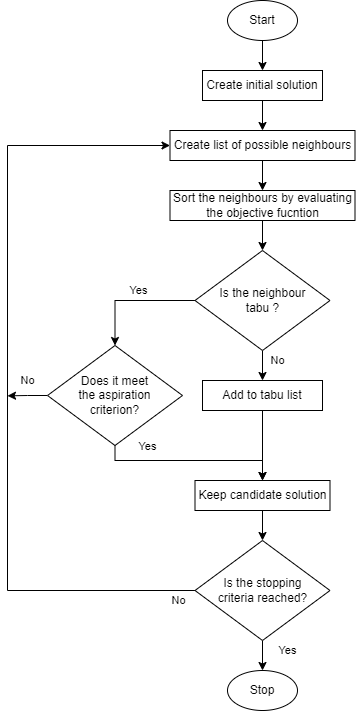
\includegraphics[width=0.5\textwidth]{images/tabu.drawio.png} 
	\caption{Tabu search flow}
	\label{fig:tabu-chart}
\end{figure}


 




%\newpage
% !TEX root = ../CedricDe Schepper2023_Thesis.tex

\section{Method}\label{sec:method}
For this thesis, the \acrlong{tabu} algorithm, as proposed by Alvarez-Valdes et al. \cite{alvarez1997}, is used to conduct our experiments. \acrshort{tabu} was chosen for several reasons. First, the simple nature of \acrshort{tabu} improves the interpretability and explainability of the method. The interpretability is important when trying to improve an algorithm based on its results. Only after understanding why a search method behaves a certain way can it efficiently be improved. High explainability makes it easier to explain the used algorithm to university administrators. Secondly, the tabu list prevents cycling between a set of states, which can reduce the amount of time needed to converge. Finally, it has been shown that \acrlong{tabu} is able to outperform other competitive algorithms  on data sets specific to institutions \cite{alvarez1997} \cite{colorni1999} \cite{Chu2000} as well as standardised benchmarks \cite{gaspero2001}.  

\subsection{Tabu Search}

 \acrfull{tabu}\cite{glover1993} starts by constructing an initial solution. The solution can be generated randomly or by applying a deterministic approach. During the entire process, both the best seen solution to date and the current solution are maintained. Keeping the best seen solution is necessary in order to allow the current solution to accept allowing worsening changes. This helps \acrshort{tabu} to avoid getting trapped in local minima. After the solution initialisation, the iterative procedure starts searching for a feasible solution. This loop ends when  a specified stopping condition is met. This condition is generally a combination of a solution its objective function scoring below a certain threshold or the procedure reaching a maximum number of iterations.
\\\\
The first step of the main loop generates the complete list of possible neighbours for the current solution and ranks them based on the objective function. Subsequently, the best neighbour, for which the required move is either not tabu or that meets the aspiration criterion, is chosen as the next solution. A move is considered tabu if it is present within the tabu list, meaning it has been used recently. The aspiration criterion is added to be able to override the tabu requirement. A possible aspiration is to accept solutions that are better than the best seen solution. After choosing the next solution, the best seen solution is updated if the newly generated solution is superior based on the objective function.
\\\\
When the stopping criteria is met, the algorithm ends and the best solution is returned. The full flow of the algorithm can be seen in figure \ref{fig:tabu-chart}.

\begin{figure}[h]
	\centering
	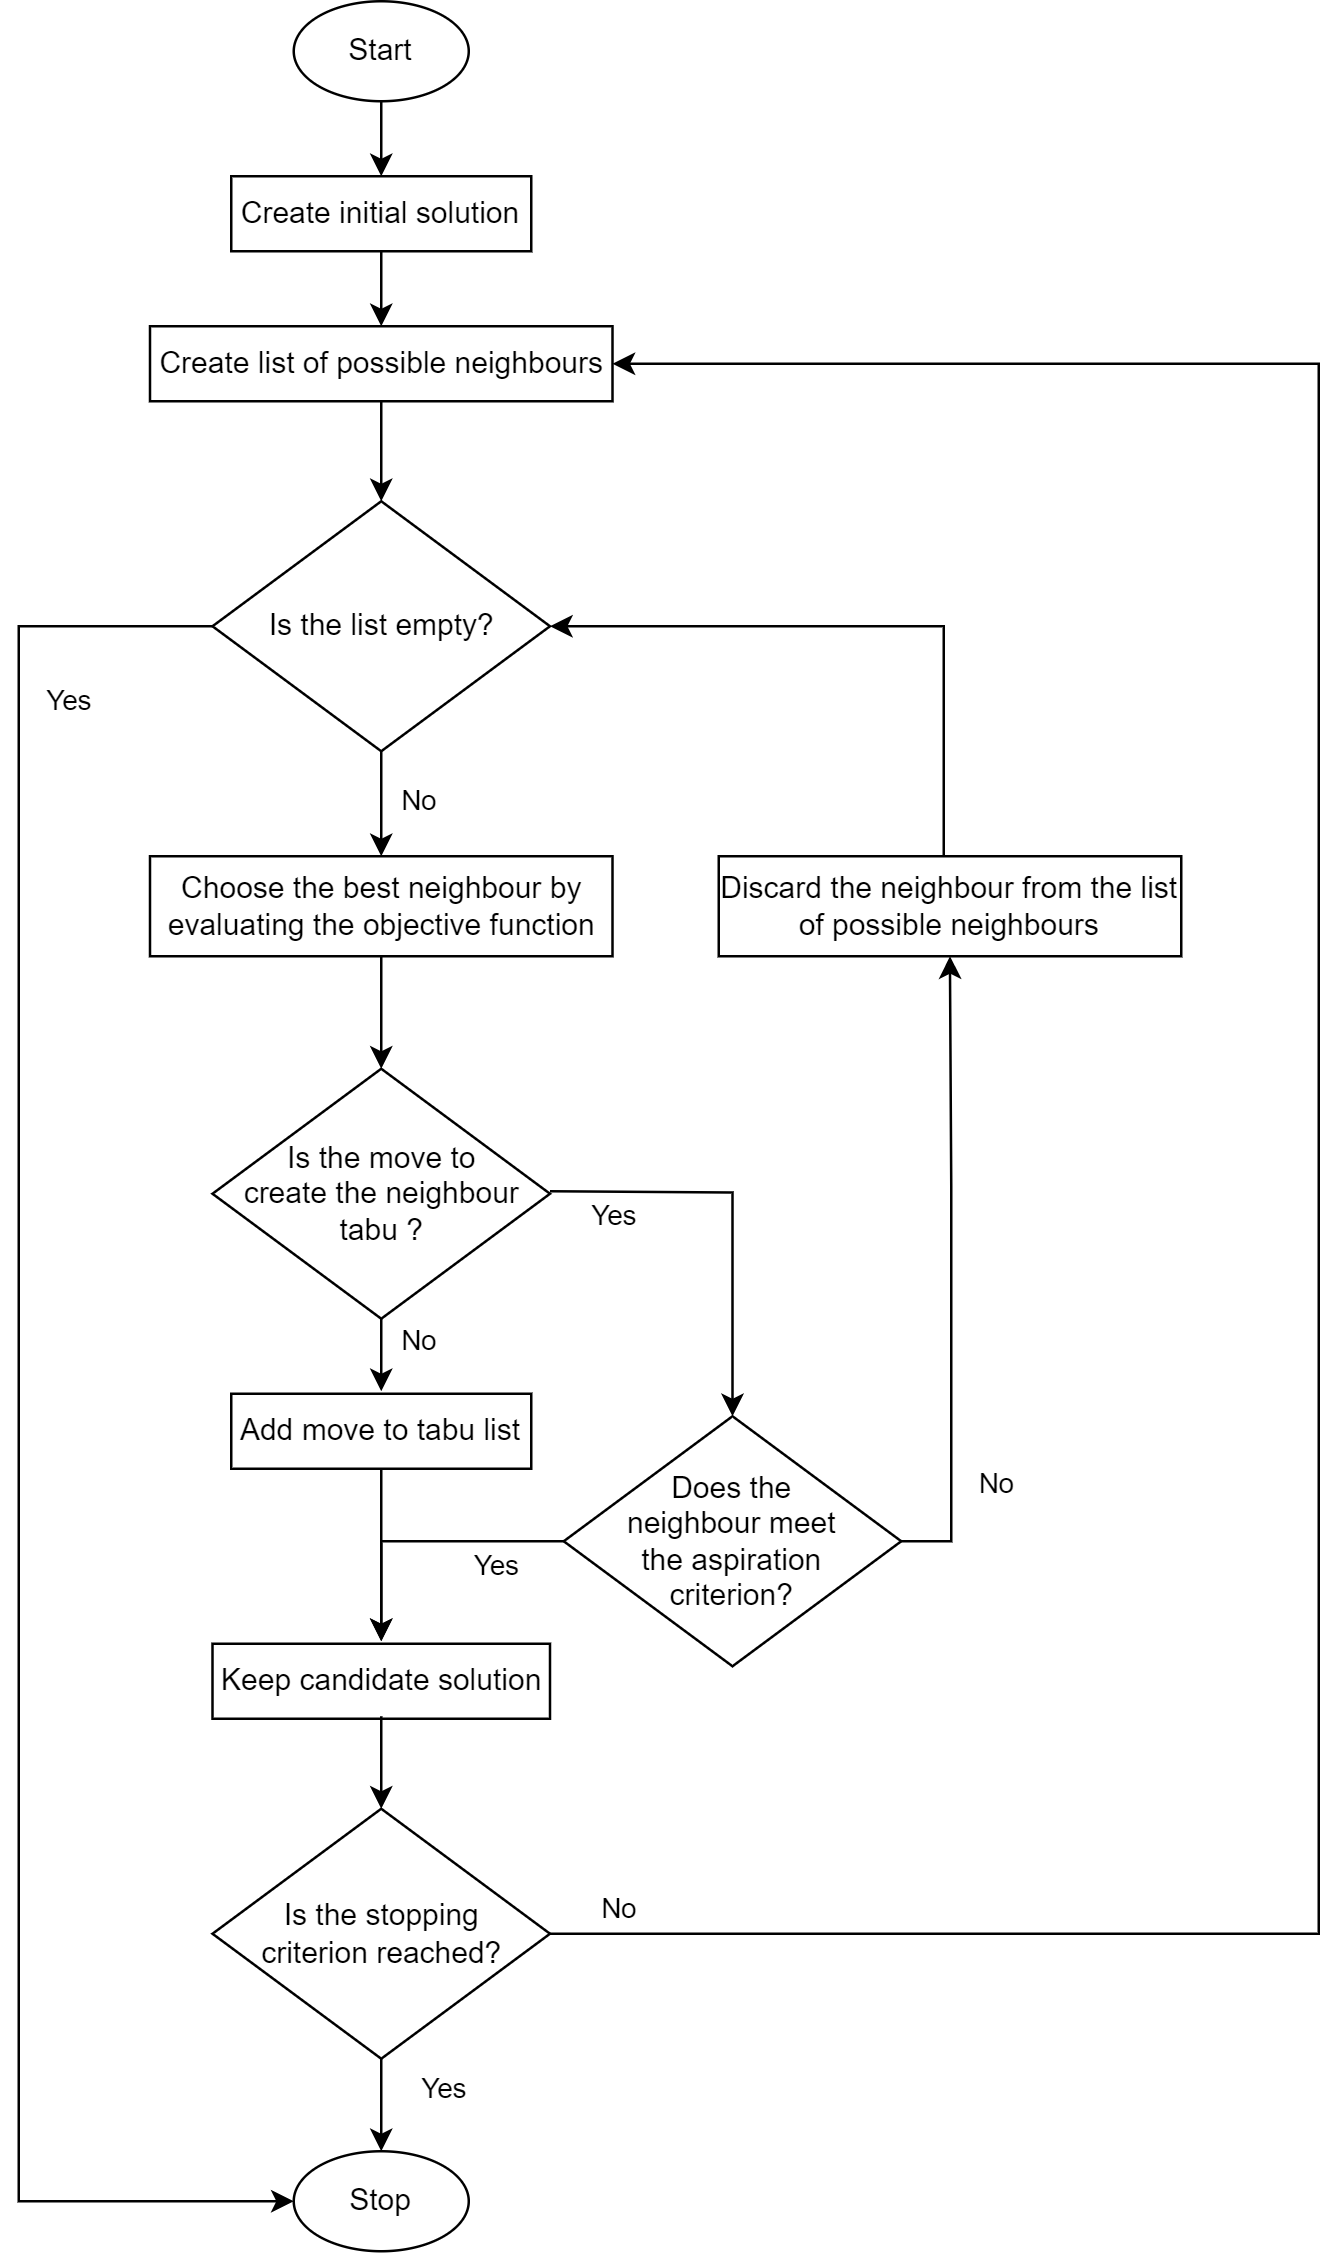
\includegraphics[width=0.8\textwidth]{images/tabu.png} 
	\caption{\acrlong{tabu} flow}
	\label{fig:tabu-chart}
\end{figure}

\subsection{Implementation frameworks}

The algorithm implemented to run the experiments is written using Python3.10. The code requires no packages that are not in the Python Standard Library. The profiler cProfiler is used to analyse the performance. It generates a list detailing how long each part of the algorithm runs for and allows to pinpoint and improve bottlenecks.

\subsection{Version 1: base algorithm}
The proposed algorithm makes use of a 2-phased approach. During phase 1, the emphasis is on the hard constraints. More specifically, reducing the amount of common students conflicts on the same day is prioritised. Optimally, this initialisation phase would return a solution that is already feasible. The second phase can be considered an optimisation phase, which tries to satisfy the soft constraints as much as possible and thus attempt to distribute the exams evenly.

\subsubsection{Initialisation phase}
The algorithm starts with the initialisation for which the pseudo code is shown in Algorithm \ref{alg:phase1}. First, the initial solution must be generated. In the proposed algorithm this is done by randomly assigning all exams to time slots. Generally, this will result in several hard constraint violations, such as students having more than 1 exam on the same day and room capacity being exceeded. Since Alvarez-Valdes et al. consider the room capacity a soft constraint, this is acceptable and will be improved during the iterations. However, in this case, room capacity is seen as a hard constraint that can't be violated at all. In order to circumvent these capacity violations, exams are sorted by student count and only then randomly assigned to time slots with rooms having sufficient capacity. As long as the time slot quantity and room capacity is sufficient, this will result in a solution with no room capacity violations. Another added complexity is the presence of different room types which was not the case for Alvarez-Valdes et al. In order to satisfy constraint 2, only rooms with a suitable type are considered when assigning exams to time slots.

\begin{algorithm}
 Generate an initial solution s in the space of solutions X\;
 $s^* = s$ (with $s^*$ the best solution seen so far)\;
 $k = 0$ (with k the number of iterations)\;
 \While{k < maximum number of iterations and $f(s^*) \neq 0$}{
  $k = k + 1$\;
  \tcc{perform single moves of one exam to another time slot}
  Generate set of solutions $V^* \subseteq N(s, k)$\ (set of neighbours of s)\;
  Sort $V^*$ by ascending $f(s')$ and select the best $s'$\;
   \ForEach{solution $s'$ in $V^*$}{
    \If{not $tabu(s')$ or $f(s') < f(s^*)$ (aspiration criterion)}{
        $s = s'$\;
        \textbf{break}\;
    }
   }
   \If{$f(s') < f(s^*)$}{
   $s^* = s'$\;
   }
 }
 \KwRet{$s^*$}

\caption{Initialisation phase}
\label{alg:phase1}
\end{algorithm}

After generating the initial solution, the iterative procedure starts by generating the set of neighbours of the current solutions. In the search space $X$, we consider a solution $s' \in X$ a neighbour of $s \in X$, whenever we can move an exam to a time slot in a different period. Evaluating the entire search space would be too time consuming. Instead, we first sort all periods by its contribution to the objective function. From the most conflictive period, we select the most conflictive time slot. Finally, we calculate all available time slots that we can swap with. In order to swap two time slots, the two affected exams (or sole affected exam when swapping to a time slot with no scheduled exam) must be able to be scheduled in the new time slots keeping the room type and capacity into account. This will ensure that no additional constraint 2 and 3 violations are introduced.

For each possible move, the objective score is calculated in order to rank all neighbours. The objective function for a solution $s$ is defined as

\begin{equation}
    f(s) = \sum_{i=1}^{P} \left( \sum_{j \in E_i}^{}\sum_{k \in E_i \atop k \neq j}^{}w \lvert S_j \cap S_k \rvert \right)
\end{equation}


with $P$ the amount of periods, $E_i$ the set of exams scheduled to period $i$, $S_j$ and $S_k$ the students scheduled to exam $j$ and exam $k$ respectively. This makes $\lvert S_j \cap S_k \rvert$ the amount of common students between the two exams. Lastly, the weight of student conflicts is denoted by $w$.

After sorting all found neighbours by objective function, the best solution, that is not tabu or for which the aspiration criterion applies, is chosen. The aspiration criterion accept a solution, for which the required move is tabu, as long as it is superior to $s^*$ (the best solution seen so far). If no moves are possible, we select the next most conflictive time slot until a suitable move has been found. When choosing the new solution, the tabu list is updated with the new tabu move consisting of the exam and period involved. Whenever the tabu list exceeds its maximum size, the oldest move is deleted, in order to allow that move again in future iterations.

Alvarez-Valdes et al. calculate the size of the tabu list as

\begin{equation} \label{eq:list}
    \text{Tabu list size} = \lfloor\sqrt{\text{\# Exams} * \text{\# Periods}}\rfloor
\end{equation}

This initialisation phase runs until a solution without conflicts has been found or the maximum number of iterations has been reached. For the latter case, the schedule will have conflicting exams during the same period with common students.

\subsubsection{Optimisation phase}

After the initialisation phase, we start the optimisation of the solution. Here the focus is including the soft constraints in the objective function to generate a solution that is the most optimal. The foundation of this phase is similar compared to the first phase with some distinct features. The overall flow can be seen in the pseudo code described in Algorithm \ref{alg:phase2}.

\begin{algorithm}
\KwData{Solution s (the result of the initialisation phase)}
 $s^* = s$ (with $s^*$ the best solution seen so far)\;
 $k = 0$ (with k the number of iterations)\;
 \While{k < maximum number of iterations and $f(s^*) \neq 0$}{
  $k = k + 1$\;
  \uIf{$k\ \mathbf{mod}\ 3 \neq 0$}{
  \tcc{perform single moves of one exam to another time slot}
    Generate set of solutions $V^* \subseteq N(s, k)$\ (set of neighbours of s after single move)\;
  Sort $V^*$ by ascending $f(s')$ and select the best $s'$\;
   \ForEach{solution $s'$ in $V^*$}{
    \If{not $tabu(s')$ or $f(s') < f(s^*)$ (aspiration criterion)}{
        $s = s'$\;
        \textbf{break}\;
    }
   }
  }
  \Else{
    \tcc{swap entire period}
    Generate set of solutions $V^* \subseteq N(s, k)$\ (set of neighbours of s after swapping periods)\;
    Sort $V^*$ by ascending $f(s')$ and select the best $s'$\;
    $s = s'$\;
  }
  
   \If{$f(s') < f(s^*)$}{
   $s^* = s'$\;
   }
 }
 \KwRet{$s^*$}

\caption{Optimisation phase}
\label{alg:phase2}
\end{algorithm}


First, the objective function is updated to take the distribution of exams into account. The objective of a solution is now defined as

\begin{equation}
    f(s) = \sum_{i=1}^{P} \sum_{j=i}^{P}\left(w_{|i-j|} \sum_{k \in E_i}^{}\sum_{l \in E_j \atop k \neq l}^{} \lvert S_k \cap S_l \rvert\right)
\end{equation}
with $P$ the amount of periods, $E_i$ the set of exams scheduled to period $i$, $S_k$ and $S_l$ the students scheduled to exam $k$ and exam $l$ respectively. This makes $\lvert S_k \cap S_l \rvert$ the amount of common students between the two exams. Here, the weight $w$ is dependent on the amount of days between the exams, with $w_i$ the weight for exams scheduled $i$ days apart.

While the objective function in the first phase only used the common students between exams during the same period, the new objective function will take all periods into account. Constraint 5a, that does not allow students having more than one exam on the same day, is now relaxed to constraint 5b. By having a large weight $w_0$ for two exams scheduled on the same day, these exam conflicts for non-model track are only introduced if the decrease of the objective function is significant. Additionally, placing exams at a further distance will now be preferred since the weight $w_{x+1}$ will be smaller than the weight $w_x$.


Secondly, two options are now available when generating the set of neighbours of the solution. The first option is a copy of the process in the initialisation phase where the set of neighbours of the solution is generated by performing single moves. Then the best solution that is either not tabu or that meets the aspiration criterion will be used. While this option might introduce constraint violations, the high $w_0$ will discourage and, depending on the values used, prevent this. This method will be alternated with a period permutation. Instead of moving a single exam, two entire periods will be swapped. Since the exams in the periods are not updated, this swap can not introduce any hard constraint violations. By moving entire periods, the objective function can change significantly in a single move. However, the amount of available moves is much lower and can be defined as
\begin{equation}
\begin{split}
   \text{\# possible moves}  & = \binom{P}{2}   \\
   & = \frac{P!}{2!(P-2)!}
\end{split}
\end{equation}

\subsection{Version 2: updating the objective function and tabu move definition}

We propose an altered version that builds on the base algorithm by changing two key aspects. First, we noticed that the objective function originally defined in the initialisation phase as   
\begin{equation}
    f(s) = \sum_{i=1}^{P} \left( \sum_{j \in E_i}^{}\sum_{k \in E_i \atop k \neq j}^{}w \lvert S_j \cap S_k \rvert \right)
\end{equation}

has an unwanted characteristic for our case: it does not punish students with several exams on the same day extra. For exam schedules without a conflict free solution, this often results in students, who are enrolled in smaller exams, having a large number of exams on the same day. In order to avoid this behaviour, the objective function is updated to
\begin{equation}
    f(s) = \sum_{i=1}^{P} \left( \sum_{s \in S(E_i)}^{}w^{c_{s,i} - 1}\right)
\end{equation}
with $P$ the amount of periods, $E_i$ the set of exams scheduled to period $i$, $S(E_i)$ the set of students with more than 1 exam during $E_i$, $c_{s,i}$ the number of exams student $s$ has on period $i$, and $w$ the weight of conflicts. By placing $c_{s,i}$ in the exponent, having multiple exams on the same day is punished severely. 

Secondly, the way a tabu move is defined was changed. Originally, when moving an exam to a different period, the combination of the exam and period was used to define the tabu move. This often resulted in the scenario that the same exam was continuously being moved. Since this generally happened to one of the largest exams, it always resulted in a large impact on the objective function and kept being presented as the most conflictive time slot. This behaviour can be avoided by having the exam as the sole identifier of the tabu move. By doing this, a single exam will not be moved as frequently.

Finally, an extra stopping criterion was added. Whenever the search finds no improvement over the best solution after 200 iterations, the search stops. This is to prevent the search taking up execution time without improving the solution. While this does not guarantee that no improvements could be discovered during later iterations, it can allow for more solutions to be generated, from which the best one can be chosen.
\subsection{Version 3: expanding the neighbourhood}

Version 1 and 2 both reduce the search space by only looking at the most conflictive time slot of the most conflictive period in order to determine the possible moves. Different time slots are only looked at when no moves are possible. This version steps away from that principle and continues evaluating the next most conflictive time slots their possible moves until a specified amount of possible moves have been found. Only then it selects the move generating the best next solution. While this increases the execution time for every iteration, more of the search space will be explored, resulting in better choices.





%\newpage
% !TEX root = ../CedricDe Schepper2023_Thesis.tex

\section{Results / Evaluation}\label{sec:results}

In order to evaluate the results from the experiment, we have to verify whether the phases perform their objective as described. Firstly, does the initialisation phase succeed in generating a `feasible´ solution namely one without or with a minimal number of hard constraint violations? Secondly, does the optimisation phase succeed in transforming the initial solution into one with an acceptable solution?

\subsection{Reference solutions}

The actual exam schedules, manually created by the administration of the \acrlong{ua}, can be used as a baseline to compare the generated schedules. These exam distributions can be seen in Figures \ref{fig:manual_sem1} and \ref{fig:manual_sem2}. Most notably, the manual schedules have a focus on keeping the amount of same day exams to a minimum and having 3+ days in between exams as much as possible. This distribution is especially visible in the schedules for \acrshort{fti}. In order to be considered a superior solution, automatically generated schedules will have to minimise the amount of exams with fewer than 2 days in between with a focus on same day exam violations.

\begin{figure}[h]
  \centering
  \subfloat[FTI]{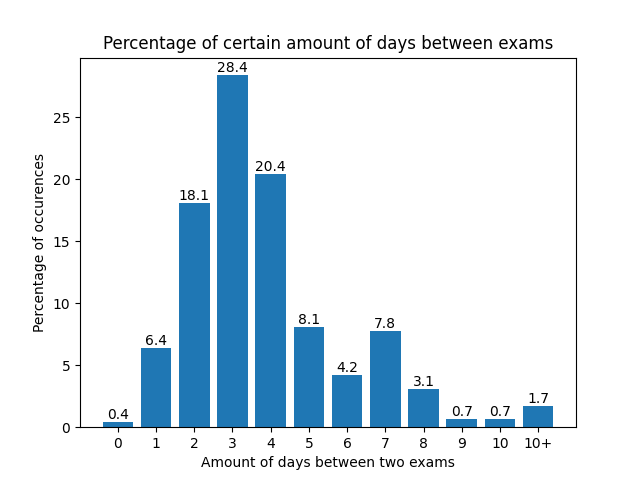
\includegraphics[width=0.5\textwidth]{images/manual/fti_sem1_percentages_manual.png}}
  \hfill
  \subfloat[FWET]{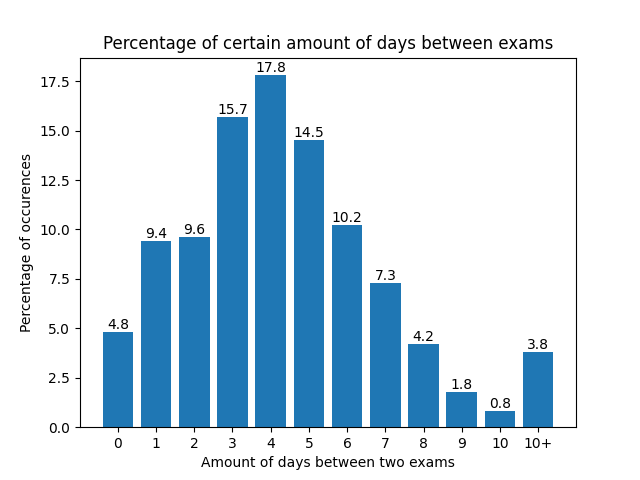
\includegraphics[width=0.5\textwidth]{images/manual/fwet_sem1_percentages_manual.png}}
  \caption{Manual exam distribution for January 2021}
  \label{fig:manual_sem1}
\end{figure}

\begin{figure}[h]
  \centering
  \subfloat[FTI]{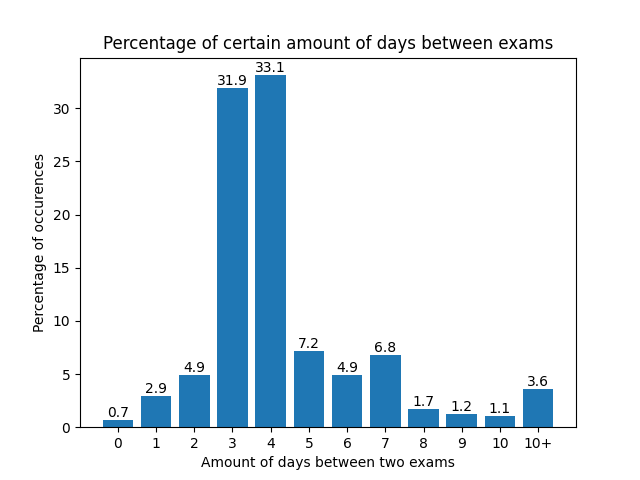
\includegraphics[width=0.5\textwidth]{images/manual/fti_sem2_percentages_manual.png}}
  \hfill
  \subfloat[FWET]{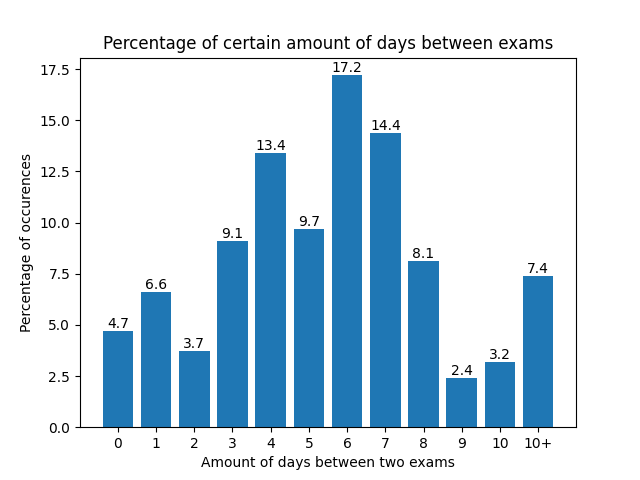
\includegraphics[width=0.5\textwidth]{images/manual/fwet_sem2_percentages_manual.png}}
  \caption{Manual exam distribution for June 2021}
  \label{fig:manual_sem2}
\end{figure}

\subsection{Initialisation phase}

In order to quantify the feasibility of a solution, it is possible to look at either the objective function or the amount of hard constraint violations. Since the objective function was adapted to contain exponents and the conflict weight having a large impact on the size of the objective, looking at the amount of hard constraint violations can provide a better perspective. By plotting the violations per iterations, the progress made by the initialisation phase can be visualised. Figure \ref{fig:violations} shows that the initialisation phase is able to generate a solution for \acrshort{fti}+\acrshort{fwet} without hard constraint violations. It reaches a feasible solution after fewer than 150 iterations, generally taking under 500 seconds. However, Figure \ref{fig:init} shows that no attention was given to the distribution which can be confirmed by the presence of a high percentage of exams after 1 day.

\begin{figure}[h]
	\centering
	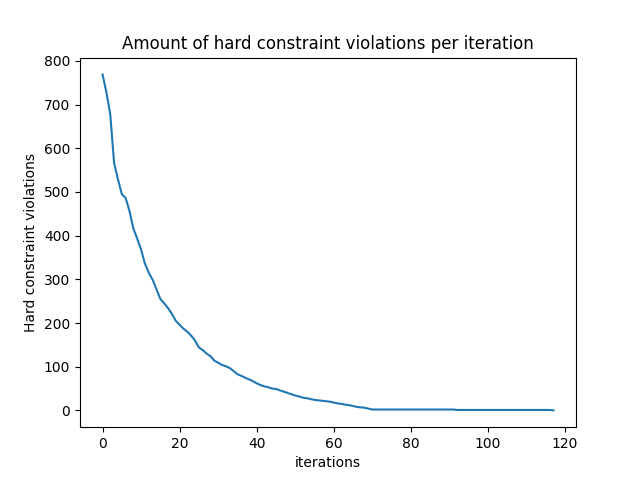
\includegraphics[width=0.5\textwidth]{images/init/conflicts.png} 
	\caption{Hard constraint violations}
	\label{fig:violations}
\end{figure}
% TODO add dotted line for y=0
\begin{figure}[h]
  \centering
  \subfloat[FTI]{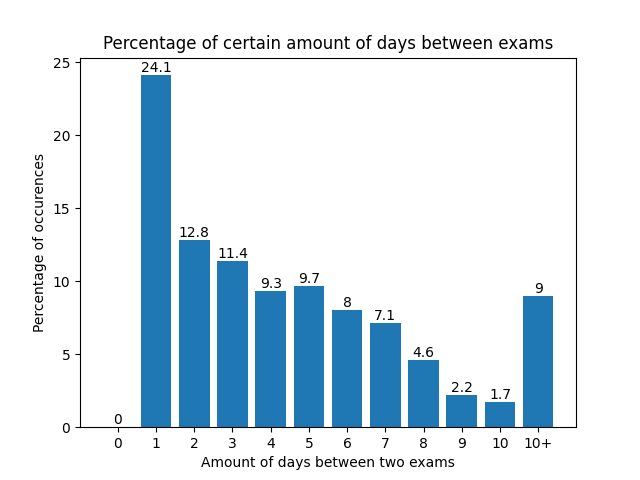
\includegraphics[width=0.5\textwidth]{images/init/fti.png}}
  \hfill
  \subfloat[FWET]{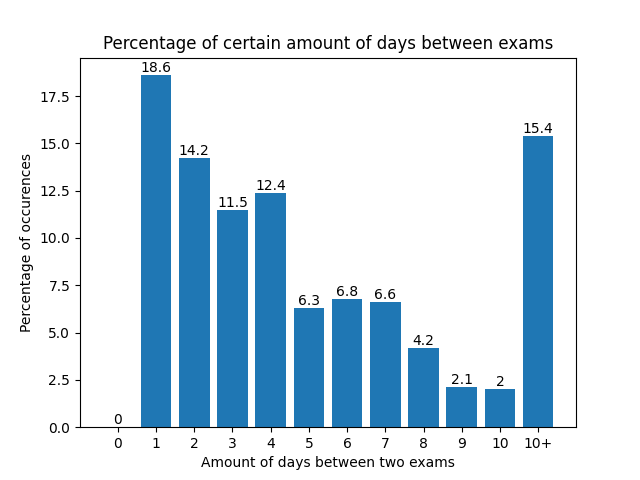
\includegraphics[width=0.5\textwidth]{images/init/fwet.png}}
  \caption{Exam distribution after initialisation phase for June 2021}
  \label{fig:init}
\end{figure}

\subsection{Optimisation phase}

While we have shown that tabu search can efficiently generate a feasible solution from the provided data set, the distribution will determine whether the automated schedules are able to beat the manual schedules. 
% Table~\ref{tab:example} shows an example of creating a table.

% \begin{table}[h]
% 	\caption{Fictitious Results}
% 	\label{tab:example}
% 	\centering
% 	\begin{tabular}{l c c c }
% 		\hline
% 		& \textbf{Precision} & \textbf{Recall} & \textbf{F-Score} \\ \hline
% 		Technique 1 & 0.85 & 0.77 & 0.81 \\
% 		Technique 2 & 0.82 & 0.81 & 0.81 \\
% 	         Technique 3 & 0.65 & 0.93 & 0.73 \\ \hline
% 	\end{tabular}
% \end{table}




%\newpage
% !TEX root = ../CedricDe Schepper2023_Thesis.tex

\section{Threats to Validity}\label{sec:threats}

In this section, we discuss the threats to the validity of the experiments performed. The presence of these threats could undermine the trustworthiness of the obtained results, and negatively affect the quality of this thesis. For every threat, we look at how we mitigated it.


% Figure~\ref{fig:threats} shows a diagram of the experiment principles and where lies each threat.
% Please do not use this image on the paper/thesis.
% Reviewers are supposed to know where the threats lie, the figure is for students to better understand the threats.
% \begin{figure}[H]
% 	\centering
% 	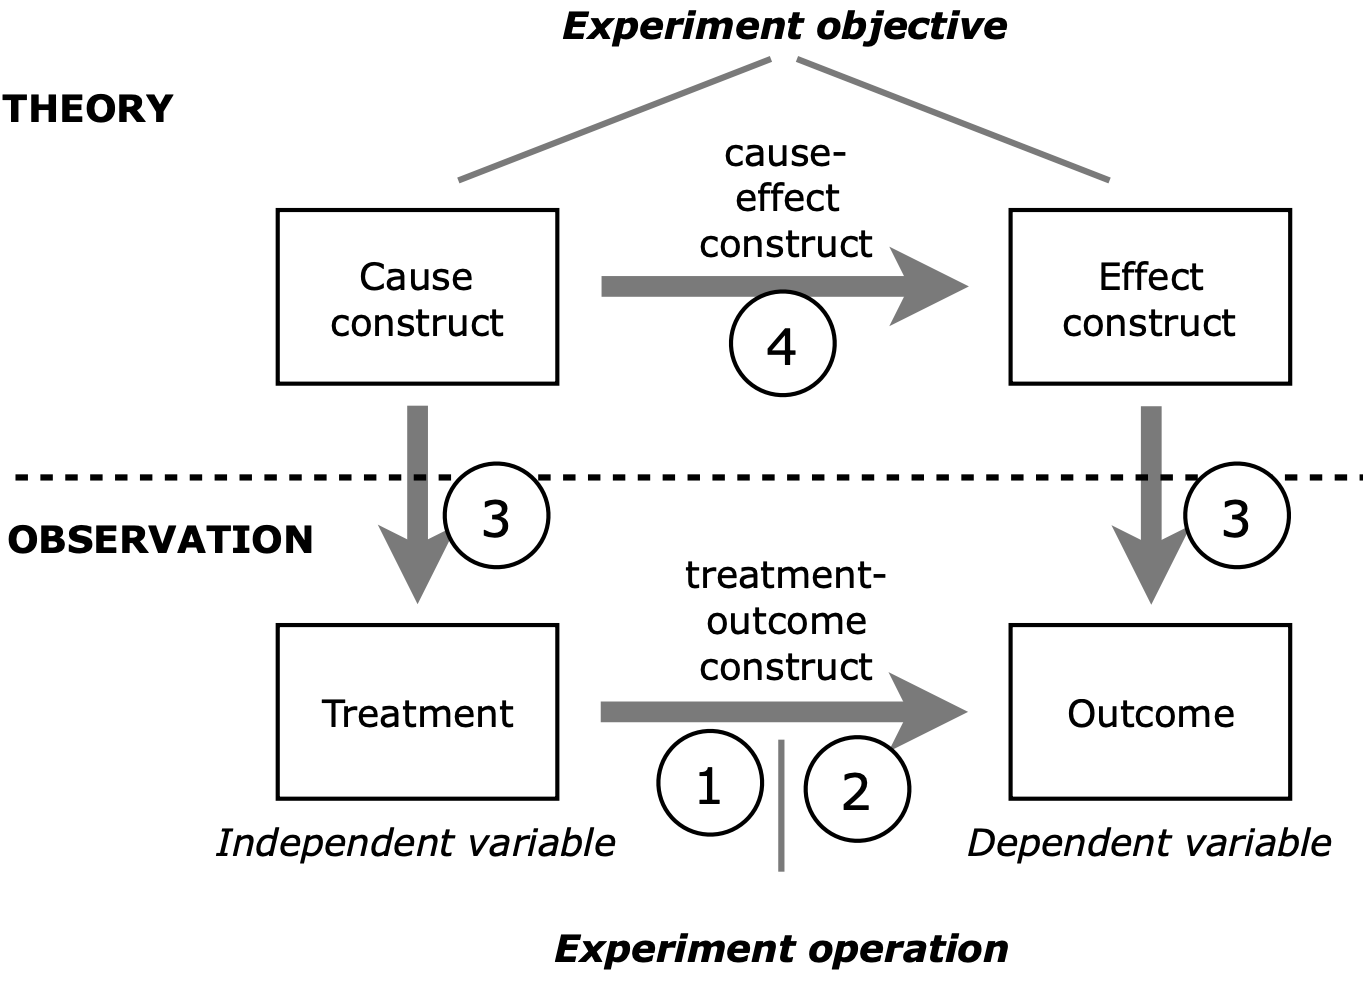
\includegraphics[width=0.75\textwidth]{images/threats-to-validity.png} 
% 	\caption{Experimental principles diagram showing threats. (1) Conclusion; (2) Internal; (3) Construct; and (4) External.}
% 	\label{fig:threats}
% \end{figure}


\subsection{Conclusion validity}

Conclusion validity refers to the reliability of the conclusions drawn from the generated results. Since only two data sets were used during the experiments, this could pose a threat to the validity of those results. However, the characteristics and size of the data set help in mitigating this threat. Both data sets consists of data from two faculties, and add up to a notable size. The size can be compared to the data set size and student workload statistics for the Toronto benchmark \cite{ceschia2022} (see Section \ref{benchmarks}). These comparison can be seen in Table \ref{tab:workload_compared}. W(avg) and W(max) detail the workload per student. These values, respectively, calculate the average and max amount of exams for every student. This shows that the size of the used data sets is competitive compared to the Toronto benchmark, especially when taking the workload into account.

\begin{table}[H]
	\caption{Student workload statistics compared between different data sets}
	\label{tab:workload_compared}
	\centering
	\begin{tabular}{l c c c c}
		\hline
		\textbf{Data set}& \textbf{Exams} & \textbf{Students} & \textbf{W(avg)} & \textbf{W(max)} \\ \hline
            \textbf{\acrfull{ua}} \\  \hline
		January 2021  & 536 & 1811 & 5.8 & 11 \\
		June 2021 & 491 & 1852 & 5.0 & 11 \\ \hline
              \textbf{Toronto benchmark instances} \\  \hline
		car91  & 678 & 16925 & 4.2 & 9 \\
		ear83 & 190 & 1125 & 7.2 & 7 \\
            hec92 & 81 & 2502 & 4.3 & 7 \\
            lse91 & 379 & 2627 & 4.2 & 8 \\
            rye93 & 485 & 9458 & 4.8 & 10 \\
            ute92 & 184 & 2672 & 4.4 & 6 \\
            yor83  & 81 & 940 & 6.42 & 14 \\ \hline
	\end{tabular}
\end{table}


% Conclusion validity is the degree to which conclusions we reach about relationships in our data are reasonable.
% \begin{itemize}
%    \item  It affects the ability to draw correct conclusion about relations between treatment and outcome. \\
% + Choice of statistical tests \\
% + Choice of sample size \\
% + Measurement of the experiment
%   \item Low Statistical Power \\
% + If power is low, there is a high risk that an erroneous conclusion is drawn.
% \end{itemize}

\subsection{Internal validity}

Threats to the internal validity of experiments risk impacting the trustworthiness of the results observed. These threats were mitigated in several ways. Firstly, the randomness in generating the initial solution helps preventing bias from infiltrating the results. Additionally, all experiments were run multiple times in order to verify that the results obtained were robust and to remove outliers. Overall, it was observed that the results after all runs produced similar results.


% Are there any other factors that may affect the results?
% \begin{itemize}
%   \item Were phenomena observed under special conditions \\
% + in the lab, close to a deadline, company risked bankruptcy, … \\
% + major turnover in team, contributors changed (open-source), …
%   \item Similar observations repeated over time (learning effects)
%   \item Correlation does not imply causation.
% \end{itemize}

\subsection{Construct validity}

The construct validity threat focuses on how accurately the scoring metrics assess the quality of solutions. The objective function and exam distribution are the two main scoring metrics used. The objective function is based on the objective function by Alvarez-Valdes et al. \cite{alvarez1997}. Additionally, the use of the exam distribution metric has been discussed and accepted as a valid metric by the University's administration in order to rate the quality of solutions.

\subsection{External validity}

The external validity threat refers to the generalisability of the findings, namely to what extend the findings can be applied to other situations. The use case presented by data and constraints of the University of Antwerp timetabling problem did not fit within any of the existing benchmarks. This could create a potential threat to the external validity of our experiments. However, the improvements applied to the original algorithm are generic in nature. For example, Version 3, as detailed in Section \ref{version3}, expands the amount of search space explored during every iteration. This expansion does not take into account any specificities of our use case and can be applied to all timetabling problems.

% A possible threat to the external validity of our experiments can be the 
% To what extent can the findings be generalized?
% \begin{itemize}
%   \item Does it apply to other languages? Other sizes? Other domains? Other systems?
%   \item Background \& education of participants
%   \item Simplicity \& scale of the team \\
% + small teams \& flexible roles vs. large organizations \& fixed roles
% \end{itemize}

%\newpage
% !TEX root = ../CedricDe Schepper2023_Thesis.tex

\section{Related Work}\label{sec:related-work}

This section details different types of algorithms researched to solve the timetabling problem. Additionally, it will also go over several benchmarks used to compare these algorithms.
%TODO expand on this


% \begin{description}
%     \item [Integer Programming] Integer Programming tries to solve an optimisation by minimising or maximising the problem's objective function. Fundamentally, some or all required variables are constrained to integers. Since integer programming makes use of an exhaustive search process, the search space must be reduced as much as possible to reduce the run time.
%     \item [Simulated Annealing] Simulated annealing\cite{kirkpatrick1983} makes use of a temperature variable which describes the level of randomness present in the acceptance of a new solution. After generating an initial solution, newly obtained solutions are accepted based on the change in objective function and current temperature. Over time the temperature cools down which reduces the amount of randomness.
%     \item [Adaptive Large Neighbourhood Search] Adaptive large neighbourhood search (ALNS) \cite{ropke2006} works by generating new solutions by constantly making changes to the current solution in order to explore the neighbourhood space. These changes are obtained by removing part of the variables and then reintroducing new values in order to generate neighbours. ALNS is considered adaptive since it keeps track of the performance of certain operations and adjusts its parameters accordingly. The use of ALNS for exam timetabling so far has been limited.
%     \item [Genetic Algorithms] Genetic algorithms (GA) \cite{Holland1975} are based on the process of natural selection witnessed in nature. They work by generating an initial set or population of possible solutions. Iteratively, a new population will be formed by selecting the fittest (best) solutions and combining two solutions to create a new generation of solutions.
%     \item [Particle Swarm Optimisation] Particle swarm optimisation (PSO) \cite{kennedy1995} is derived from the behaviour by collective species as seen in fish schools and bird flocks. A swarm of particles (see fish or bird), representing solutions, moves through the search space at a certain speed and direction.
%     \item [Honey-Bee Mating Optimisation] Honey-bee mating optimisation algorithms (HBMO) \cite{abbas2001} are based on the mating of honey-bees as witnessed in nature. During the mating procedure, the queen representing the current best solution is able to mate with other bees in order to produce new solutions.
%     \item [Great Deluge] Great deluge algorithms (GD) \cite{dueck1993} are based on the principle where an increasing water level is used to represent the allowed threshold. Only a solution that is superior in comparison with that threshold is accepted.
%     \item [Hyper-heuristics] Hyper-heuristics\cite{cowling2001} are designed to be problem-independent meaning no domain expertise and customisation is needed to be successfully applied to different problems. These heuristics utilise the heuristic the most optimal for the given problem.
% \end{description}
Several classes for optimisation methods exists, all with their own unique characteristics. Algorithms from the following classes are covered in this section:
\begin{description}
\item [Single Solution-based Meta-heuristics]

Single Solution-based Meta-heuristics are also commonly referred to as \acrfull{local} methods \cite{lin1973}. These heuristics first generate an initial solution. Afterwards, small changes are continuously applied to the solution using a specific strategy in order to traverse the search space. 

They can often be divided into either one-stage or two-stage algorithms \cite{lewis2008}. One-stage methods attempt to satisfy both the hard and soft constraints during the same stage. Two-stage approaches initially only take the hard constraints into account in order to generate a feasible solution. Afterwards, the second phase attempts to optimise the solution by adding the soft constraints. Since \acrshort{local} methods only accept a solution when its better than the previous one, encountering a worse solution blocks it from progressing. This means that \acrshort{local} requires strategies in order to escape local optima to keep improving the solution. 

% discuss the many parameters?


\item [Population-based Meta-heuristics]

Instead of applying meta-heuristic on a single solution, Population-based meta-heuristics maintain a set of solutions, called a population. Every iteration, a new population is generated by applying meta-heuristics. These methods offer the advantage over single solution-based methods that multiple solutions are presented during the final iteration. Another difference is that they prioritise exploration of the search space while single solution-based methods focus more in exploitation of their solution  \cite{kohshori2012}. However, this exploration does come at the cost of an increase in run time due to a larger amount of operations applied at each iteration.

\item [Exact Methods] 

Exact methods constrain the problem by defining a linear objective function and force some or all parameters to be integers. Since these methods make use of an exhaustive search process, the search space must be reduced as much as possible to reduce the run time. Unlike heuristics, exact methods can provide upper and lower bounds of the objective function and thus provide proof of optimality.

Fundamentally, some or all required variables are constrained to integers. 

\item [Hyper-heuristics]

Hyper-heuristics\cite{cowling2001} \cite{burke2013} are designed to be problem-independent meaning no domain expertise and customisation is needed to be successfully applied to different problems. They utilise the heuristic the most optimal for the given problem.

\end{description}

\subsection{Standardised data sets and benchmarks}

Even though the timetabling problem has been tackled in many research papers, Ceschia et al.\cite{ceschia2022} state that many of the initial benchmarks are not relevant anymore. They observe that many papers do not provide the data, source code or solutions used. This makes it impossible to confirm the presented results. Additionally, many of the problems researched are unique to specific institutions, reducing the amount of relevant observations that can be made from the results. However, effort has been put into standardising the timetabling problems into data sets that can be used to accurately compare different heuristics. The agreement regarding the need for benchmarks dates back to the first \acrfull{patat} in 1995 \cite{cumming1995}. Most of the current benchmarks available come from competitions like the \acrfull{itc}.

An early formulation for university exam timetabling was done by Carter et al. \cite{carter1996}. They initially introduced 13 exam timetabling data sets for several institutions, commonly referred to as the Toronto or Carter benchmarks. Additional instances have been made available over time \cite{bellio2021}. The data behind this format is implemented as a binary enrolment matrix, showing for each exam and student whether the student is enrolled for that exam. The objective function to compare solutions for this benchmark is based on the distance between exams and the amount of common students. The penalty for two exams with $k$ common students at a distance of $i$ periods was calculated as $k*w_{i}$. The values for $w_1$, $w_2$, $w_3$, $w_4$, and $w_5$ were set as $16$, $8$, $4$, $2$, and $1$, respectively. While this benchmark is still being used to compare heuristics, the simplification of several common constraints means that it less suitable to apply on real-world scenarios. For example, the benchmark is considered to be uncapacitated. This means that exam rooms are not taken into account when generating timetables. Since constraint 2 determines room capacity to be nonnegotiable in our use case, our timetabling problem does not fit in this format.

A later examination timetabling formulation was proposed for ITC-2007 by McCollum et al. \cite{mccollum2007}. This formulation is more advanced than the one proposed by Carter et al., taking more constraints into account. New constraints include the addition of exam rooms and more strict penalties related to the distance of scheduled exams. Initially, a data set of 12 instances was released for the competition but more real-world instances have been translated to the format over time \cite{parkes2010}, as well as the implementation of a generator to create artificial instances \cite{battistutta2017}.

Other common benchmarks focus on either the high school or university course scheduling problem. For example, Post et al. \cite{post2012} were the first to propose a standardised format for  high school timetabling. They developed XHSTT, an XML format to be used in solution benchmarks. Several data sets have been made available at \url{https://www.utwente.nl/en/eemcs/dmmp/hstt/}.
Additionally, this format has been used as the target for the third International Timetabling Competition in 2011. Unfortunately, university exam timetabling problems do not allow to be converted into course timetabling formats due to differences in constraints and schedule characteristics. Other examples include the \acrfull{cb-ctt} \cite{gaspero2007} and \acrfull{pe-ctt} \cite{lewis2007} formats, both used for ITC-2007.

These problem formulations provide valuable contributions in standardising the timetabling research, allowing for easier comparison between algorithms and checking of solutions. However, the uniqueness of the use cease for the University of Antwerp makes using these benchmarks infeasible. This makes it possible to only compare the quality of generated solutions against the ones manually generated.

\subsection{Single Solution-based Meta-heuristics}

Single Solution-based Meta-heuristics or \acrlong{local} methods start from an initial solution. Generally, this solution is generated randomly or using a greedy algorithm, but other techniques can also be used. \acrshort{local} then starts exploring the search space by calculating the neighbourhood of its current solution and picking a neighbour as its new solution. Different versions of \acrlong{local} use their own technique for choosing the neighbour and when to stop the search. The objective function is used to estimate the quality of each solution, with \acrshort{local} attempting to miminise this objective.
\subsubsection{Tabu Search}

\acrfull{tabu} \cite{glover1993} is based on \acrfull{local} \cite{lin1973}, meaning it traverses the possible search space by performing local changes to the current solution. Since \acrshort{local} will only accept improving solutions, this traversal can end up being stuck in a local optimum. \acrshort{tabu} differs from \acrshort{local} by relaxing this rule and also accepting worsening solutions. This relaxation allows for more exploration and allows \acrshort{tabu} to escape local optima. Additionally, \acrshort{tabu} maintains a memory structure to avoid changes being reversed. The usage of short- to long-term memory is  based on the assumption that optimisation techniques must incorporate memory to qualify as intelligent and that a bad strategic choice is superior to a good random choice\cite{glover1999}. This memory structure is implemented by maintaining a tabu list which contains the x most recent changes performed. A change is thus considered ‘tabu’ if it is present within the tabu list.

Alvarez-Valdes et al. \cite{alvarez1997} proposes a two-phased \acrlong{tabu} in order to solve the university exam timetabling problem. During
the first phase, the emphasis is on satisfying the hard constraints. More specifically, they attempt to reduce the amount of occurrences where a student has two exams on the same day. Optimally, this initialisation phase would return a solution that is already feasible. The second phase can be considered an optimisation phase, which tries to satisfy the soft constraints as much as possible and thus attempt to spread the exams as best as possible. They used this algorithm on real-world data sets of the University of Valencia, and compared it with the manually designed exam schedules. They conclude that the generated schedules are superior for all data sets.

Di Gaspero and Schaerf \cite{gaspero2001} adapt the original \acrshort{tabu} method by proposing changes to the tabu list and stopping criterion. Instead of keeping a fixed tabu list size, each move is assigned a number of iterations that the move is considered tabu. Additionally, the algorithm will terminate after a fixed amount of iterations without improvement. When comparing their results with the Carter benchmarks, they note that \acrlong{tabu} provides comparable performance with the benchmarks.

Chu and Fang \cite{Chu2000} made a comparison between using \acrlong{ga} versus \acrlong{tabu} to obtain time tables. For all of their different experiments, the \acrfull{tabu} implementation was able to outperform their \acrshort{ga} version, both on the quality of the solution and the computational time needed to converge. However, a redeeming quality of \acrlong{ga} is that they are able to produce several near optimal solutions in one go while \acrlong{tabu} implementations are limited to a single solution. 

Colorni et al. \cite{colorni1999} apply \acrlong{tabu}, \acrlong{sa}, and \acrlong{ga} on the high school timetabling problem for an Italian high school. They conclude that \acrshort{tabu} outperforms both competitors in generating quality timetables for their use case.



\subsubsection{Simulated Annealing}

Aycan and Ayav \cite{aycan2009} apply \acrfull{sa} \cite{kirkpatrick1983} to generate optimal solutions. In order to create a initial solution as optimal as possible, constraint satisfaction methods are used to create a solution satisfying all hard constraints. During the simulated annealing phase, a new solution is found by randomly swapping two variables. The cost of the new solution is then calculated using the objective function. Whenever the new objective is lower than the objective of the previous solution, the algorithm will keep the new solution. In the case of a higher objective, the temperature will determine based on the difference between the two costs whether to keep the new solution or discard it. The possibility of accepting worsening solutions allows the algorithm to avoid being stuck in local minima. Over time the temperature will reduce based on the cooling schedule. Practically, the allowed difference in cost for worsening solutions in order to still be accepted will decrease. As the temperature decreases, the focus switches from exploring to exploiting the search space. This will allow the algorithm to eventually converge towards a local or global minimum. The performance of simulated annealing is determined by the choice of initial solution, the objective function, and cooling schedule. 

The objective function accounts for the impact of both hard as well as soft constraints. Every constraint is assigned its own penalty function including a constraint weight. The cooling schedule proposed makes use of geometric schedule. That means that the temperature will decrease by a constant factor during every step of the algorithm. The choice for the initial temperature and cool-down factor will determine the share of the search space visited. 

While geometric cooling is very simple to implement, it has some shortcomings. Since the temperature is calculated by a deterministic schedule, it mostly depends on the variables chosen by the user. Additionally, this schedule also does not take into account the progress made by the algorithm. Alternatively, more complex adaptive cooling schedules will decrease, or even increase, the temperature based on the rate of acceptance for new solutions. While Aycan and Ayav conclude that this method succeeds in satisfying the hard constraint in order to find a feasible solution, implementing a hybrid version or adding reheating to the cooling schedule might obtain higher quality results.
% TODO data set

A more complex cooling schedule can be seen in the \acrfull{sar} algorithm by Leng Goh et al.\cite{Goh2017}. They propose a two stage hybrid timetabling algorithm where the first stage uses \acrlong{tabu} to generate a feasible solution. If such a solution is found, the second stage attempts to improve on it by using \acrshort{sar}. Instead of using geometric cooling, reheating or increasing the temperature is possible. This is based on the assumption that whenever the objective is high, the focus should be on exploration and accordingly whenever the objective is low, exploitation is prioritised. Whenever the search is estimated to be stuck in a local optima, the temperature will be reheated until it manages to escape. 

This estimate is made by checking the difference between the best and current objective. If the change in objective is under a certain threshold for a pre-determined amount of iterations, the search is considered to be stuck and reheating will occur. This cooling and reheating repeats itself until an optimal solution has been found or a step limit is reached. An additional benefit to reheating compared to a geometric schedule is that no fine-tuning of variables is needed when extending the run time. Figure \ref{fig:SAR} showcases the effect that enabling reheating has on the temperature, with its value increasing whenever it gets stuck in a local optimum. As a consequence, the search is allowed to explore more, resulting in a higher amount of variation of the objective. In this case, the reheating allowed the search to discover a more optimal solution.
% TODO data set

\begin{figure}[h]
  \centering
  \subfloat[\acrshort{sar} with reheating disabled]{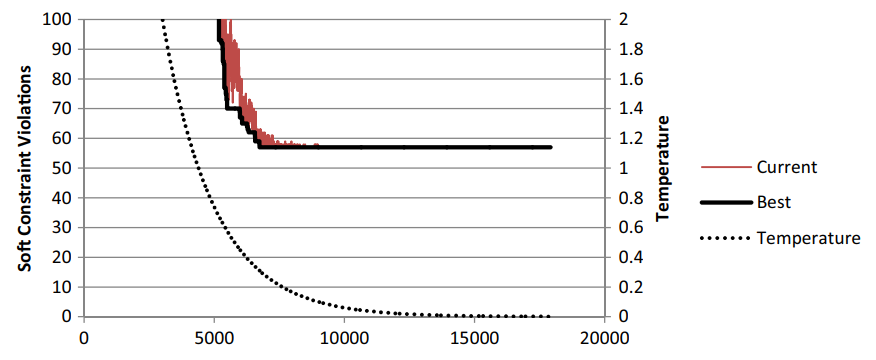
\includegraphics[width=0.5\textwidth]{images/related_works/SA/SAR_disabled.png}}
  \hfill
  \subfloat[\acrshort{sar} with reheating enabled]{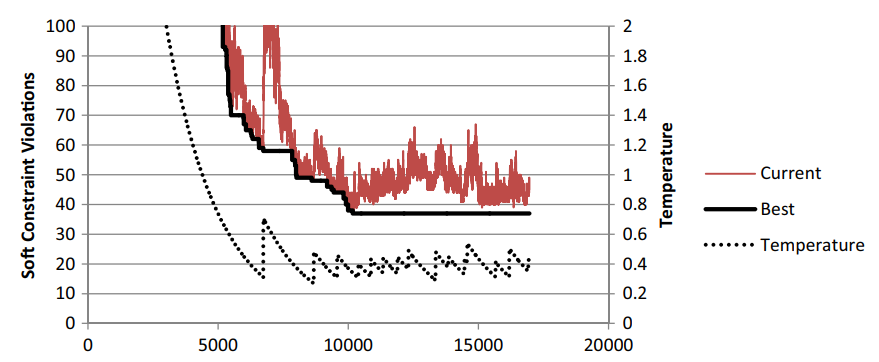
\includegraphics[width=0.5\textwidth]{images/related_works/SA/SAR_enabled.png}}
  \caption{Effect of reheating on the temperate and objective for \acrlong{sa} as discovered by Leng Goh et al.\cite{Goh2017}}
  \label{fig:SAR}
\end{figure}





\subsubsection{Adaptive Large Neighbourhood Search}

\acrshort{alns} \cite{ropke2006} works by generating new solutions by constantly making changes to the current solution in order to explore the neighbourhood space. These changes are obtained by removing part of the variables and then reintroducing new values in order to generate neighbours. ALNS is considered adaptive since it keeps track of the performance of certain operations and adjusts its parameters accordingly. 

S{\o}rensen and Stidsen \cite{sorensen2012} propose a version of \acrshort{alns}, building on the more general \acrfull{lns} algorithm. \acrshort{lns} works by creating new solutions by applying a "destroy" and "repair" operation. Every step a destroy operation will remove a set of variables from the problem, before reintroducing new variables in order to create new solutions. By changing multiple variables, \acrshort{lns} is able to escape local minima. In the proposed \acrshort{alns} extension however, the single destroy and repair operations are replaced by multiple operations, chosen at random during execution. This changes the original deterministic model into a stochastic version, introducing randomness. Additionally an adaptive layer analyses the impact of each operator and increases the probability of operators having a positive impact on the objective function.

\subsubsection{Great Deluge}

Dueck \cite{dueck1993} first proposed a \acrfull{gd} algorithm as alternative to \acrlong{sa}. It is built on the principle that the search space is limited by an ever changing water level. Newly generated solutions are only considered whenever they are superior compared to the objective threshold level that is represented by the water level. New solutions are found by performing low-level heuristics such as swapping two exams. While Dueck makes use of a simple linear function to determine the water level, different functions can be applied instead. While \acrlong{sa} accepts worsening solutions based on a probabilistic value, \acrshort{gd} has a hard cut-off point for accepting solutions. 

% something about the 
Burke et al. \cite{burke2004GD} are the first to apply an algorithm based on \acrlong{gd} to the exam timetabling problem. Their reason for using \acrshort{gd} is to be able to control the exact run time of the search while still allow the search to converge. While this could be done with the \acrlong{sa} algorithm for example, determining the exact cooling rate for a correct execution time is often too complex. Instead they propose a \acrshort{gd} implementation that they call a degraded ceiling algorithm. Instead of a changing water level, they describe a lowering ceiling with the ceiling representing the upper boundary of the objective function allowed. By slowly moving the ceiling down, the run time before convergence can be accurately determined. This is valuable for university administrators responsible for creating exam timetables since they could let the search run overnight or during the weekend.

By slowly lowering the ceiling, exploration to worsening solutions is feasible as long as the ceiling level has not cut off certain sections of the search space. As the ceiling lowers, the search space becomes tighter and priority shifts to exploitation. This continues until no further improvement is feasible and the stopping criterion is met. They conclude that this degraded ceiling implementation is not only superior to a time limited simulation annealing version, but that running this algorithm for long periods can produce extremely good results. Based on their experiments, degraded ceiling can outperform most algorithms whenever a long run time is feasible.

Kahar and Kendall \cite{kahar2015} propose an modified \acrlong{gd} algorithm where the water level or decay rate is dynamically changed. Whenever no improvements are found, the change in water level can be reversed in order to allow more exploration. Based on their experiments using data from Universiti Malaysia Pahang, the modified \acrshort{gd} algorithm outperforms both the university's proprietary software and the original algorithm by Dueck \cite{dueck1993}. Lnasya Syafitrie and Komarudin \cite{Lnasya2022} implemented their own version based on this modified algorithm, with the main change being a slower rate at which the water rises. They find that their version outperforms that of Kahar and Kendall.

%Section 4 + modified algo (good paper)
%Kahar and kendall
%https://www.tandfonline.com/doi/abs/10.1057/jors.2012.169?journalCode=tjor20
%https://sci-hub.st/https://doi.org/10.1057/jors.2012.169

McMullan \cite{mcmullan2007} has implemented the \acrlong{gd} algorithm with the addition of a reheating step, similar to the reheating used for \acrlong{sar} \cite{Goh2017}. This better allows the search to escape local optima. While the general \acrshort{gd} algorithm would terminate after observing no improvement for an amount of time steps, the extended will apply a one-time reheating, reducing the water level again. this allows certain worsening solutions to be accepted again resulting in a larger possible search space. Afterwards the decay rate is increased compared to the initial rate. Experiments using small, medium, and large benchmark data sets show that the extended GD algorithm outperforms other implementations such as \acrlong{local} and ant algorithms on the medium data sets. For the small and large data sets, no notable difference is noted.


\subsection{Population-based Meta-heuristics}
\subsubsection{Genetic Algorithms}

\acrfull{ga} \cite{Holland1975} are based on the process of natural selection witnessed in nature. It generally consists of several base steps before reaching a final solution. First, the algorithm creates an initial population consisting of feasible solutions. An iterative approach is then taken in order to evolve this population into new generations. For every generation, the fitness of each individual in the population is determined and the 'fittest' individuals are chosen as parents for the new generation. In order to obtain new offspring, genetic operators such as crossover and mutation are applied. Crossover works by combining information of parent solutions into a new offspring. This can be done by swapping exam assignments across the parents. Mutation on the other hand randomly changes assignments in order to create new offspring. This is done in order to maintain randomness, allowing \acrshort{ga} to escape local minima. The flow of \acrlong{ga} can be seen in Figure \ref{fig:GA}.

\begin{figure}[h]
	\centering
	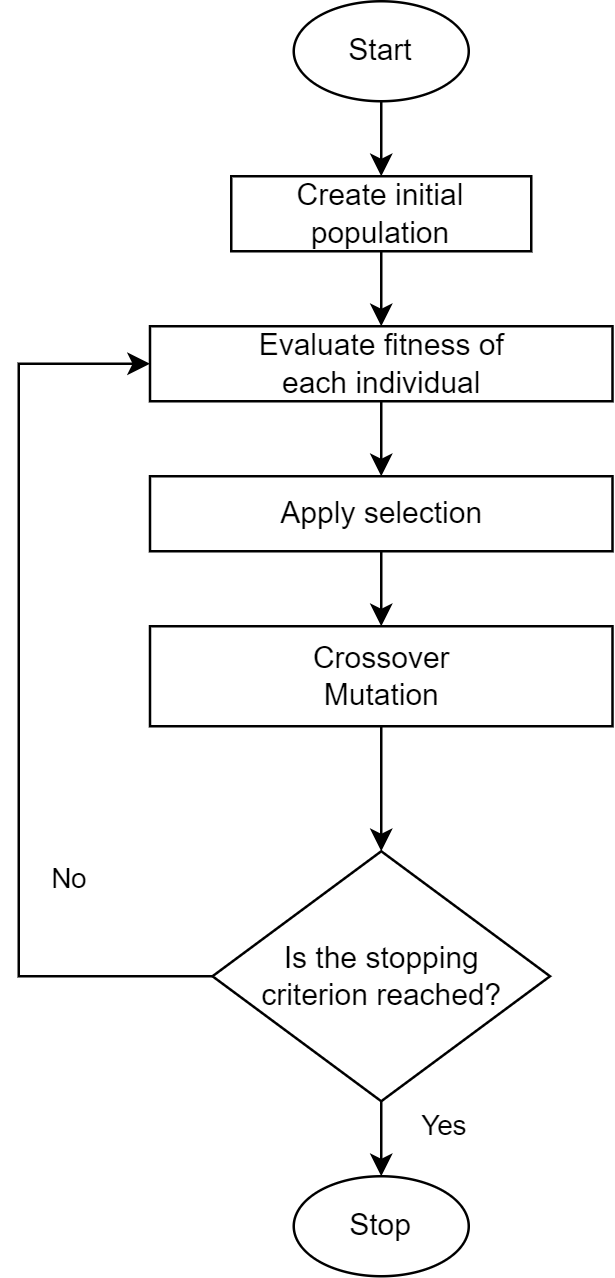
\includegraphics[width=0.40\textwidth]{images/related_works/GA/GA.png} 
	\caption{\acrlong{ga} flow}
	\label{fig:GA}
\end{figure}

The paper submitted by Pillay and Banzhaf \cite{pillay2010} showcases a two-phased approach to create feasible timetables. Both phases utilise a \acrshort{ga} implementation in order to come to a solution, with the first phase focusing on producing a timetable that does not violate any hard constraints. The second phase later attempts to optimise the objective of the soft constraints. Up until 2007, most papers applying \acrshort{ga} used data sets specific to a particular institution. This algorithm is tested on the Carter benchmarks \cite{carter1996}, allowing its performance to be compared to different approaches.

During the first phase, domain specific heuristics are used instead of random operations in order to create the initial population. While these heuristics require domain knowledge, the quality of the initial population should be superior. In order to determine the next exam to be assigned, the obtained heuristics make use of the number of conflicts, the number of students enrolled per exam, or the number of students with conflicts. These heuristics were then compared to random and best-slot scheduling. It was found that using heuristics succeeded in lowering the soft constraints objective compared to other scheduling methods. For the iterative steps, the fitness function is described as the amount of conflicts per timetable. In order to select the parents with which to generate the new generation, tournament selection is applied. Here, a determined amount of individuals are randomly chosen from the population to be compared against each other. The individual having the lowest objective ends up being selected. This process is repeated until all parents have been selected. When creating new offspring, both mutation and crossover operators were considered. During mutation, a random amount of conflicting examinations are rescheduled. Moreover, crossover operations that randomly swap time slots between two parents were tested. This requires an additional repair mechanism to remove duplicate examinations and schedule missing examinations. However, they note that the crossover operations applied did not positively impact the quality of the solutions. For the final implementation, only the mutation operation on single parents is used to create offspring.

The second phase focuses on minimising the objective of the soft constraints in order the generate a more optimal timetable. While very similar to the first phase,  mutation operations are now continuously applied until an offspring superior to the parent is found or until a certain amount of iterations has been reached. The performance of this genetic algorithm was eventually compared to other studies using the same benchmark including \acrlong{tabu} and l\acrlong{lns}. While no optimal solutions were found for any of the data sets, equal or improved solutions were obtained compared to alternative methods. They conclude that their implementation equals or even outperforms other evolutionary algorithms on the Carter benchmarks.

\subsubsection{Particle Swarm Optimisation}

\acrfull{pso} \cite{kennedy1995} is derived from the behaviour by collective species as seen in fish schools and bird flocks. A swarm of particles (see fish or bird), representing solutions, moves through the search space at a certain speed and direction.
% TODO: expand on this?

Chen and Shih \cite{Chen2013} discuss a \acrlong{pso} implementation combined with \acrlong{local}. During \acrshort{pso}, a swarm of particles, corresponding to different timetables, moves through the available search space. During every iteration, each particle will remember its best encountered position and share its information with the rest of the swarm. The particles will then adjust their velocity and direction on both their personal and global best. The velocity can be seen as the magnitude of the allowed change per time step. Additionally, a local search iteration is applied to explore the surrounding space for a better solution. In order to avoid particles being trapped in a local optimum, a disturbance operation is introduced \cite{tsai2010}. This operation forces particles to move towards unexpected directions, that aren't based on previous experience. Doing this, the amount of exploration is increased.
% TODO data set

Tassopoulos and Beligiannis \cite{Tassopoulos2012} builds on the general \acrlong{pso} algorithm. Initially, they start with a high amount of 150 particles. Whenever the fitness value of a produced particle exceeds a certain tolerance value, this particle is set to inactive and will not be used in further steps. This tolerance value is calculated during each step in order to deactivate weak particles at the start but make it harder for particles to reach that threshold down the line. When the amount of particles is reduced to 30, this procedure stops. The reasoning behind starting with a large amount of particles is to make it possible to explore a wider search space while keeping the execution time down by reducing the particles over time. Similar to Chen and Shih's approach \cite{Chen2013} a \acrlong{local} algorithm is used to minimise one of the soft constraints. Results show that it outperforms the \acrfull{ga} implementation that their \acrshort{pso} version was tested against.
% TODO data set
\subsubsection{Honey-Bee Mating Optimisation}

\acrfull{hbmo} \cite{abbas2001} are based on the mating of honey-bees as witnessed in nature. During the mating procedure, the queen representing the current best solution is able to mate with other bees in order to produce new solutions. Since specific terms used in the natural mating process are used when describing the optimisation algorithm, Table \ref{tab:hbmo} provides translation of the analogy. \acrshort{hbmo} follows the natural process when the queen leaves the hive on a mating flight. Here she maintains a certain speed and direction, creating the possibility of drones to mate with her. After mating with a drone, its genetic information is stored within the queen to be used in the breeding phase. After each mating, the queen will change her energy and speed. As soon as the queen reaches a certain energy threshold or reaches a mating limit, she will return to the hive. Upon return, the queen will randomly select genetic information obtained and perform a crossover step to create a new brood. Every brood is fed by a worker in order to improve the obtained solution. After every brood is improved, the fittest brood is compared to the queen. If the brood corresponds to a superior solution, the queen is replaced by the brood. Both the queen and the other broods are killed and a new mating flight will commence. 

Sabar et al. \cite{Sabar2009} are the first to propose the use of \acrlong{hbmo} in order to solve the exam timetabling problem. The proposed variant on the original algorithm \cite{abbas2001} attempts to solve \acrshort{hbmo}'s weakness of suffering from early convergence. Originally, the drones, that are used to mate with the queen, are never replaced which reduces the amount of variation. This is solved by replacing the drones that were successful in mating with the newly created broods. Additionally, after crossover, the heuristic applied by the worker is based on \acrlong{local} in order to optimise the brood as much as possible.

While \acrshort{hbmo} is very similar to other population based methods such as genetic algorithms, two clear differences can be noted. First, \acrshort{hbmo} maintains the queen as one of the two 'parents' used during crossover. Since the queen is considered as the current best solution, this is meant to improve obtained solutions. Secondly, the \acrlong{local} applied by the worker can be considered an exploitation phase which is not present in \acrlong{ga}. Finally, Sabar et al. conclude that the proposed \acrshort{hbmo} alternative manages to create comparable or superior solutions compared against other population-based methods.

\begin{table}[h]
	\caption{Analogy between the natural mating process and the \acrshort{hbmo} algorithm}
	\label{tab:hbmo}
	\centering
	\begin{tabular}{l c c }
		\hline
		\textbf{Natural honey bee}  & \textbf{Artificial honey bee} \\ \hline
		Queen & Current best solution \\
		Drones & Possible solutions \\
	    Broods & Newly generated solutions \\
            Worker & Heuristic search \\
            Mating or Breeding & Crossover \\ \hline
	\end{tabular}
\end{table}

% TODO data set

\subsection{Exact Methods}
\subsubsection{Integer Programming}

Kristiansen et al. \cite{kristiansen2015} describe a \acrfull{mip} model designed to solve XHSTT timetabling data sets. The XHSTT format was formulated to standardise timetabling data sets in order to compare heuristics. The proposed model makes use of two stages. During the first stage, a simplified \acrshort{mip} model is generated taking only the hard constraints of the problem into account. This stage is ran until a specified amount of time has passed or until the model has been solved to optimality. The benefit of using integer programming here is that \acrshort{mip} models can issue 'certificates of optimality, indicating that an optimal solution has been reached. This differs from heuristic methods where a model cannot guarantee that an optimal solution has been found unless the objective function is brought to 0. With \acrshort{mip} models, one can determine whether the cost generated by the hard constraints is the most optimal solution feasible. This allows a clear cut off point for the model to stop focusing on the hard constraints solely. 

If a certificate of optimality can be generated, the second stage is executed. Otherwise, the algorithm ends. Before solving the model in stage 2, the soft constraints are added again. Additionally, an extra constraint is added which keeps the optimal value of the cost generated by the hard constraints. The second stage ends after the remaining time after stage 1 has passed. The proposed model was not only successful in creating 2 new solutions to XHSTT data sets, it was also able to prove optimality of previously found solutions. Additionally, it could also provide the lower bounds for several other data sets and improve the best solution found so far. These lower bounds are crucial in order to compare the quality of solutions that have not reached optimality.
% TODO data set

Al-hawari et al. \cite{hawari2017} attempts to solve the university exam timetabling problem by splitting the problem into three smaller sub-problems in order to significantly decrease the amount of variables required in the formulas used and thus reduce the processing power and storage capacity needed. Additionally, the simplification of the formulas also improves the explainability of the model, making it easier to understand. The initial problem is split into 3 problems, each sub-problem continuing on the solution provided by the previous phase. Phase one and two will use a  graph colouring \acrfull{ip} model to generate a feasible solution. Graph colouring works by assigning colours to the vertices while avoiding that two vertices connected by an edge are assigned the same colour. These vertices are called adjacent. Additionally, graph colouring will attempt to use the least amount of colours possible to generate a feasible solutions.

The first phase starts by assigning time slots to the different exams. Different from stated in the problem definition, Al-hawari et al. consider a time slot to be a moment in time when exams are being held. For example, during an exam period of 20 days with two exam moments a day, there would be 40 time slots available for exams to be planned. Initially, these time slots are solely an exam moment and do not include a day yet. During the first phase, exams are seen as the vertices with two vertices being connected by an edge if a student is enrolled in both exams. The time slots act as colours and are assigned to the vertices. Every feasible solution produced by this phase will satisfy the hard constraint that a student can not have more than one exam at the same time. Phase two builds upon this solution by assigning days to the time slots, meaning that the time slots are now considered vertices and the different days colours. Again, vertices are adjacent if the exams assigned to the time slots share mutual students. The new solution will have added the extra constraint that a student can't have two exams on the same day. Lastly, the third stage will assign all exams to rooms, keeping into account the exam enrolment and room capacity. The final solution, if feasible, will satisfy all hard constraints. An important remark to note is that no soft constraints were introduced for creating an improved exam distribution. As a result, a feasible solution will only make sure that a student has no exams on two following days or on the same day.
% TODO data set


\subsection{Hyper-heuristics}

While many optimisation methods have proven successful in generating optimal solutions, many of these methods are designed for a single problem and require domain-specific knowledge to be efficient. Hyper-heuristics attempt to solve this problem by providing a problem-independent solution which allows different methods to be used across problems. They can be considered either selective or generative. Selective hyper-heuristics choose from a predefined set of heuristics depending on the problem encountered, while generative hyper-heuristics procure new heuristics by combining multiple heuristics.

Kheiri and Keedwell \cite{kheiri2017} focus on the selection hyper-heuristics to solve the high school timetabling problem. Every iteration in the solution process, consists of two steps. First, low-level heuristics are applied. These heuristic apply basic operations to create new solutions. Secondly, a move acceptance method will determine whether the keep or discard the new solution. In their study, a set of 15 low-level heuristics are employed including randomly rescheduling or unscheduling an exam, shuffling the time slots of several exams, changing the room of an exam,.... For the move acceptance method, several methods such as Hill Climbing, \acrlong{sa} and, \acrlong{gd} are compared. The choice of acceptance method will determine when a new solution is accepted. In hill climbing, a solution will only be accepted if its better compared to the previous solution. On the other hand, in \acrlong{sa}, worse solutions can be considered due to the probability determined by the temperature.

The hyper-heuristic proposed by Kheiri and Keedwell proposes a sequence-based selection where each time a sequence of heuristics is applied instead of a single heuristic. Experiment results show that these sequences outperform single applications of heuristics and that the selection of the low-level heuristics is more important than the move acceptance method used. They finally conclude that the proposed method provides solutions superior to those of previous popular methods.

Kendall and Mohd Hussin \cite{kendall2004} describe a hyper-heuristic where the order of the low-level heuristics applied to the current solution is determined by a \acrlong{tabu} implementation. At each step of the search, the heuristic with the best performance, if not tabu, is chosen to explore its own search space. The heuristics chosen then become tabu, which means that they will not be considered in the next iterations. Because of this, the search space of other low-level heuristics that might perform worse will also be explored. The size of the tabu list becomes a variable to be optimised for each problem instance. The same set of 13 low-level heuristics proposed during one of their previous experiments was reused \cite{kendall2005}. Kendall and Mohd Hussin conclude that the hyper-heuristic is able to find solutions that are 80\% better compared to manual generated solutions based on their objective function.





%\newpage
% !TEX root = ../CedricDe Schepper2023_Thesis.tex

\section{Conclusions}\label{sec:conclusion}

 In this thesis, we investigated how an implementation of the \acrlong{tabu} search method compares to manual generated timetables. Due to constraints such as the requirement for different exam room types and the notion of model track students, we were unable to copy existing implementations that proved successful in recent benchmarks. 

 The experiments performed show that the \acrshort{tabu} implementations were able to generate solutions without any exam conflicts. In order to provide a better final exam distribution, we successfully improved the \acrshort{tabu} implementation, proposed by Alvarez-Valdes et al.\cite{alvarez1997}. These changed reduced the percentage of occurrences where a student has two or fewer days between exams. For both the January and June data set, this distribution improved from 33.3\% to 27.3\%, and from 23.9\% to 15.2\%, respectively.
 
When comparing the generated solutions to the reference solutions, the proposed implementation was able to reduce the amount of exam conflicts from nearly 3\% to zero or close to zero. However, the change in objective function was not able to effectively change Constraint 5 into a soft constraint, in order to improve the overall distribution. For the January 2021 data set, 27.9\% of the time a student had two or fewer days between exams, while the reference solution was superior with only 12\%. The same was visible for June 2021, with 15.4\% versus the 11.9\% of the reference solution.

In conclusion, we laid the foundation for further research by formalising the requirements enforced by the university's administration into hard and soft constraints. Additionally, we provided an algorithm, that is capable of creating time tables without exam conflicts. These time tables can then be used as initial solutions, from which to continue manual improvement. This combination would reduce the amount of time spent while keeping the flexibility observed during manual creation.

Based on the scheduling problem defined, future research could investigate the performance when implementing different search methods. Additionally, the search problem can be further expanded by increasing the amount the amount of constraints present. For example, by adding constraints specific to certain exams, such as an exam requesting a specific room.



% \begin{itemize}
% \item \textbf{Summary of Results.} 
%    In a paper/thesis, we probably have many pages in previous sections presenting results. 
%    Now in the conclusion, it is time to put the most important results here for the reader. 
%    Especially research with measurable results, we highlight the numbers here. 
% \item \textbf{Main Findings / Conclusions.} 
%    Many times, we have a result but based on its number we can draw a conclusion or formulate a finding on top of it. 
%    Even if it was previous discussed in an earlier section, we need to re-state here. 
% \item \textbf{Contributions.} 
%    If we presented/discussed the main contributions of this research in the introduction, then we need to do again in the conclusion.
%    Do not repeat verbatim what was written in previous sections. 
%    In the conclusion, we expect contributions to be more detailed and linked to the results/findings when possible.
% \end{itemize}

% Avoid generic conclusion sentences that could be applied to anything. 
% For example, "Our technique showed good results which were beneficial to answer our research questions. 
% Our work can be used by other researchers to better understand our domain."
% Instead, go for more specific detailed results.
% For example, "Our technique showed a precision of 75\% which was 15\% higher than the baseline comparison. 
% Based on this we can see that ..."

% The final paragraph (or paragraphs) of the conclusion is about future research. 
% We can create a separate subsection for it if there are multiple paragraphs dedicated to future work. 
% Just be aware, it is not a good sign if future research content is longer than what we wrote for the previous paragraphs in the conclusion.


\newpage
\bibliographystyle{unsrt}
\bibliography{references}
\addcontentsline{toc}{section}{References}

\end{document}